\documentclass{article}
\usepackage[utf8x]{inputenc}
\usepackage{ucs}
\usepackage{amsmath} 
\usepackage{amsfonts}
\usepackage{marvosym}
\usepackage{wasysym}
\usepackage{upgreek}
\usepackage[english,russian]{babel}
\usepackage{graphicx}
\usepackage{float}
\usepackage{textcomp}
\usepackage{hyperref}
\usepackage{geometry}
  \geometry{left=2cm}
  \geometry{right=1.5cm}
  \geometry{top=1cm}
  \geometry{bottom=2cm}
\usepackage{tikz}
\usepackage{ccaption}
\usepackage{multicol}
\usepackage{hyperref}

\makeatletter
\def\@bignumber#1#2{%
  \ifx#2\end
    #1\let\next\@gobble
  \else
    #1\hspace{0pt plus 1pt}\let\next\@bignumber
  \fi
  \next#2}
\newcommand{\bignumber}[1]{\@bignumber#1\end}
\makeatother

\usepackage{listings}
%\setlength{\columnsep}{1.5cm}
%\setlength{\columnseprule}{0.2pt}

\usepackage[absolute]{textpos}

\begin{document}
\pagenumbering{gobble}

\lstset{
  language=C,                % choose the language of the code
  basicstyle=\linespread{1.1}\ttfamily,
  columns=fixed,
  fontadjust=true,
  basewidth=0.5em,
  keywordstyle=\color{blue}\bfseries,
  commentstyle=\color{gray},
  stringstyle=\ttfamily\color{orange!50!black},
  showstringspaces=false,
  numbersep=5pt,
  numberstyle=\tiny\color{black},
  numberfirstline=true,
  stepnumber=1,                   % the step between two line-numbers.        
  numbersep=10pt,                  % how far the line-numbers are from the code
  backgroundcolor=\color{white},  % choose the background color. You must add \usepackage{color}
  showstringspaces=false,         % underline spaces within strings
  captionpos=b,                   % sets the caption-position to bottom
  breaklines=true,                % sets automatic line breaking
  breakatwhitespace=true,         % sets if automatic breaks should only happen at whitespace
  xleftmargin=.2in,
  extendedchars=\true,
  keepspaces = true,
}
\lstset{literate=%
   *{0}{{{\color{red!20!violet}0}}}1
    {1}{{{\color{red!20!violet}1}}}1
    {2}{{{\color{red!20!violet}2}}}1
    {3}{{{\color{red!20!violet}3}}}1
    {4}{{{\color{red!20!violet}4}}}1
    {5}{{{\color{red!20!violet}5}}}1
    {6}{{{\color{red!20!violet}6}}}1
    {7}{{{\color{red!20!violet}7}}}1
    {8}{{{\color{red!20!violet}8}}}1
    {9}{{{\color{red!20!violet}9}}}1
}
\title{Семинар \#1: Основы. Домашнее задание.\vspace{-5ex}}\date{}\maketitle
\subsubsection*{Задача 1 - Продвинутый helloworld:} 
Вывести на экран строку \texttt{!\textbackslash@\#\$\textasciicircum\&\%} Если возникнут вопросы по этой или по другим задачам, то ответы можно найти на stackoverflow. Просто загуглите, например, "how to print backslash c stackoverflow".

\subsection*{Цикл \texttt{for}:}
Цикл \texttt{for} - это просто более удобная запись цикла \texttt{while}. Например, код, который печатает все числа от \texttt{1} до \texttt{100} через пробел с помощью циклов \texttt{while} и \texttt{for}:
\begin{center}
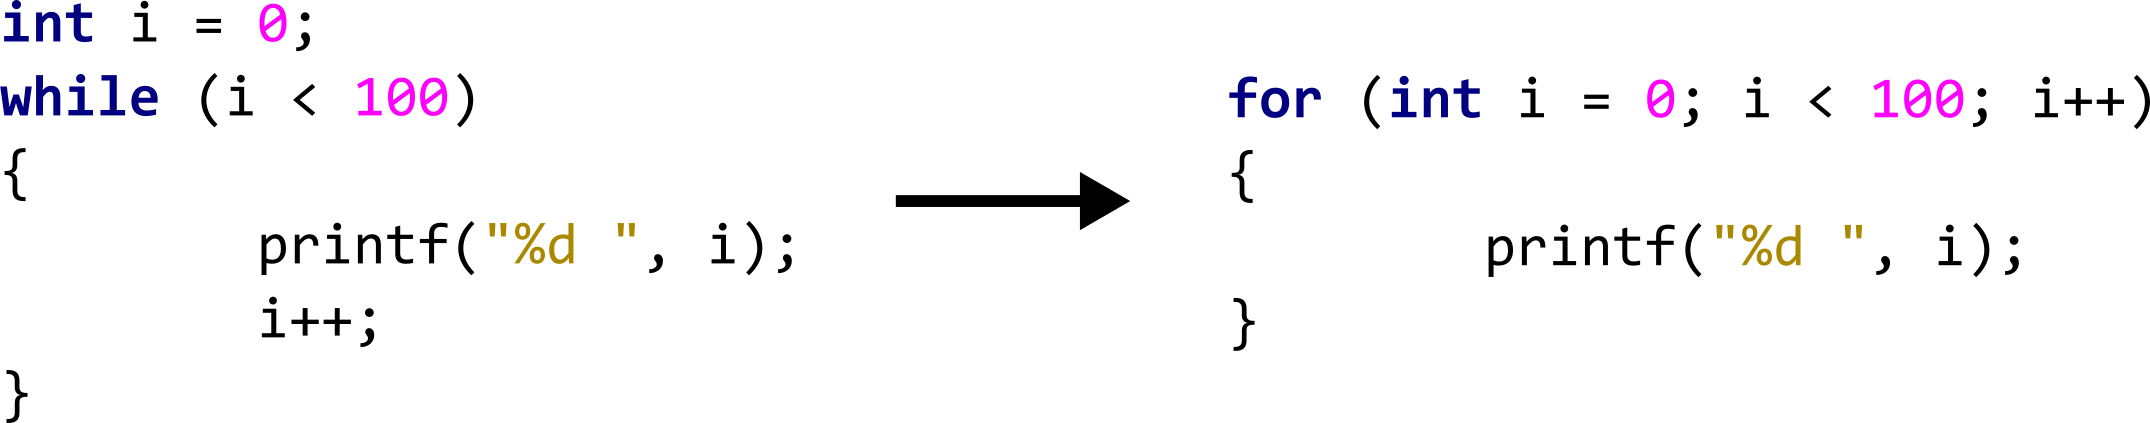
\includegraphics[scale=0.9]{../images/whilefor.png}
\end{center}

\subsubsection*{Задача 2 - Число, квадрат и куб:} 
Напишите программу, которая будет печатать само число, его квадрат и его куб от \texttt{1} до \texttt{n}, разделённые стрелочкой.
Число \texttt{n} считывается с помощью \texttt{scanf}. 
Например, при \texttt{n = 5}, программа должна напечатать следующее:
\begin{verbatim}
1 ->  1 ->   1
2 ->  4 ->   8
3 ->  9 ->  27
4 -> 16 ->  64
5 -> 25 -> 125
\end{verbatim}

\subsubsection*{Задача 3 - Таблица умножения:} 
Напишите программу, которая будет печатать таблицу умножения в виде квадратной таблицы (такую же, как печатают на задней стороне тетрадей). Используйте 2 вложенных цикла \texttt{for}.

\subsection*{Целочисленные переменные:} Различные целочисленные типы языка C представлены в следующей таблице:

\begin{center}
\begin{tabular}{ c c c c }
 тип & размер (байт) & диапазон значений ($2^{\# bits}$) & спецификатор \\ \hline
 char & 1 & от -128 до 127 & \%hhd \\ 
 short & 2 & от -32768 до 32767 & \%hd  \\  
 int & 4 & примерно от -2-х миллиардов до 2-х миллиардов & \%d  \\  
 long & 4 или 8 & такой же как у int или long long в зависимости от системы & \%ld  \\  
 long long & 8 & примерно от $-10^{19}$ до $10^{19}$ & \%lld  \\  
 unsigned char & 1 & от 0 до 255 & \%hhu \\ 
 unsigned short & 2 & от 0 до 65535 & \%hu  \\  
 unsigned int & 4 & примерно от 0 до 4-х миллиардов & \%u  \\  
 unsigned long & 4 или 8 & такой же как у unsigned int или unsigned long long & \%lu  \\  
 unsigned long long & 8 & от 0 до $2^{64} \approx 2*10^{19}$  & \%llu  \\  
 16-ричная система & - & - & \%x  \\ 
 указатель & 8 & $2^{64} \approx 2*10^{19}$ & \%p  \\  
\end{tabular}
\end{center}



\subsubsection*{Задача 4: Арифметика char:}
Стандартный тип \texttt{char} - это целые числа, размером в 1 байт. Ниже приведён пример программы, в которой используются числа типа \texttt{char}. Что напечатает программа? Объясните результат (нужно прислать словесные объяснения по значению каждой переменной). 
\begin{lstlisting}
#include <stdio.h>
int main()
{
	char a = 100;
	char b = a + 50;
	char c = 2 * a;
	char d = a * a;
	unsigned char e = 2 * a;
	printf("%hhd %hhd %hhd %hhd %hhu\n", a, b, c, d, e);
}
\end{lstlisting}

\subsubsection*{Задача 5: Произведение чисел:} Напишите функцию, которая вычисляет произведение 2-х положительный чисел $a < 2^{32}$ и $b < 2^{32}$. Проверьте вашу функцию на следующих значениях:
\begin{center}
\begin{tabular}{ c c }
 вход & выход \\ \hline
 2 2 & 4  \\ 
 2000000000 2 & 4000000000  \\ 
 1444444444 777777777 & 1123456788654320988 \\ 
 4222222222 3777777777 & 15950617279827160494 \\   
\end{tabular}
\end{center}
\subsubsection*{Задача 6: Факториал:} Напишите функцию, которая вычисляет факториал числа $n \leq 20$ (при больших значениях \texttt{n} факториал не влазит даже в \texttt{unsigned long long}). Проверьте вашу функцию на следующих значениях:
\begin{center}
\begin{tabular}{ c c }
 вход & выход \\ \hline
 0 & 1  \\ 
 1 & 1 \\  
 5 & 120   \\  
 10 & 3628800   \\  
 20 & 2432902008176640000   \\  
\end{tabular}
\end{center}

\subsubsection*{Задача 7: Размещения:} В комбинаторике размещением (из n по k) $A_n^k$ называется упорядоченный набор из k различных элементов из некоторого множества различных n элементов. Размещения вычисляются следующим образом: $A_n^k = \frac{n!}{(n-k)!}$. Напишите функцию, которая будет вычислять размещения при условии, что  $A_n^k < 2^{64}$. Проверьте вашу функцию на следующих значениях:
\begin{center}
\begin{tabular}{ c c }
 вход & выход \\ \hline
 5 2 & 20  \\ 
 20 10 & 670442572800  \\ 
 30 12 & 41430393164160000 \\ 
 60 11 & 13679492361575040000 \\   
\end{tabular}
\end{center}


\subsubsection*{Задача 8\textbf{*}: Последняя цифра числа Фибоначчи:} Найдите последнюю цифру \texttt{n}-го числа Фибоначчи.
\begin{center}
\begin{multicols}{2}
\begin{tabular}{ c c }
 вход & выход \\ \hline
 1 & 1  \\ 
 2 & 1  \\ 
 6 & 8 \\  
 20 & 5 \\   
 123 & 2 \\   
\end{tabular}
\begin{tabular}{ c c }
 вход & выход \\ \hline
 987 & 8 \\  
 1234567 & 3  \\ 
 123456789 & 4 \\  
 12345678987654321 & 6 \\
 12345678987654321777 & 2 \\   
\end{tabular}
\end{multicols}
\end{center}
\end{document}